\section{Project Management} \label{sec:pm}
\todo[inline, color=yellow]{Laura}
In this section the planning and the management of the \textit{Interactive Lighting Lab} is described. As there were only two persons involved in this project the following part is going to be a bit more compressed than the reader might expected it.\\
To give the customer an all-encompassing idea about the \textit{Interactive Lighting Lab} a project proposal was handed in, which is written in German. It is divided in two sections. First of all a motivation is given and afterwards the exercise, which should be implemented is determined. It is translated into English and can be found in section~\ref{sec:ProjectProposal}. \\ 
Before starting the actual project it is wise to make some mindful project plans in order to organize the project. First of all a catalogue of requirements and specifications (compare section~\ref{sec:PMcatalogue}) was written to formulate all important basic information of the project. \\
The project structure plan, which is presented in section~\ref{sec:StructurePlan}, serves to arrange the work packages of the project in a sorted way. The relating milestone description can be found in section~\ref{sec:Milestones}. \\
For staying in time while the implementation phase, a time exposure is required (compare section~\ref{sec:timeExposure}).\\
A list with all early detectable risks can be found in the table in section~\ref{sec:risks}.\\
In section~\ref{sec:pmCon} a final resume about the changes during the actual realisation of the project is given. 


\subsection{Project Proposal}\label{sec:ProjectProposal}
\todo[inline, color=yellow]{Laura}

\textbf{Motivation} \\
Due to progressive changes in image processing programs and high-resolution images, the manipulation of digital images has became easier. A common form of manipulation is the so-called "\textit{image splicing}". Therefore image regions of at least two images where combined to a new one. The transitions between the individual image parts can get invisible for the user by using accurate and user-friendly image processing tools.
According to \cite{Hsu2006DetectingIS} there is still no algorithm, which makes images completely forgery-proof by adding watermarks to it. There is put much effort in the integrity of images and the recognition of manipulated image parts, despite the lack of prior knowledge of the image content. This should be improved by the \textit{Interactive Lighting Lab}. An algorithm should be established, which proofs the consistence in light directions on various surfaces presented on an image. The light vectors will be conveniently estimated to give an assertion on whether the image is manipulated or not.\\

\textbf{Work Steps} \\
Until now there is no implementation given by \textit{OpenCV}, which estimates the light vector of an infinite light source on one surface and compares it with the according vector of another surface in the same image. An approach in the programming language \textit{C++} should be implemented using the assumptions of Johnson and Farid \cite{Johnson} to compute, analyse and visualize the light vectors. \\The following work stages are necessary: 

\begin{itemize}
\item Creation of test images with an infinite light source, e.g. in nature on a sunny day 
\item Implementation of a GUI for the visualisation of the approach
\item Implementation of the algorithm of Johnson and Farid \cite{Johnson}
\item Optional: The approach might be amended by also taking a local (not infinite) light source into consideration \cite{Johnson}
\end{itemize}


\subsection{Catalogue of Requirements and Specification} \label{sec:PMcatalogue}
\todo[inline, color=yellow]{Laura}
Project Manager: Laura Anger \\
Team Member: Vera Brockmeyer \\
Supervisor: Prof. Dr. Dietmar Kunz\\ \\
\textbf{Project Goals}\\ \\
This project aims to implement an interactive image forensic tool to detect lighting detections of various objects in an image. The tool is limited to images with infinitive light sources. All resulting direction vectors are compared with each other to give a statement if the image is partly digital modified.\\
 
The development of the tool requires the following parts: 
\begin{itemize}
\item a set of test images with a simulated infinitive light source
\item an interactive partial contour detection tool 
\item a calculation and validation of lighting detection vectors 
\item a graphic user interface which includes Live-Wire and visualisation tools
\end{itemize}

The project will be realised in the programming languages C++ with the OpenCV, the Dlib C++ Library and the Qt Library. The release of the project is planned on 4th August 2017. \\

\textbf{List of Requirements}\\

\underline{Set of Test Images}

A set of ten test images is required to validate the image forensic tool. These images have to be captured with an simulated infinitive light source. Thus, all image are taken at a sunny day with no cloudy heaven. Each image shows either different types of objects with surfaces and contours like reflecting metal and glass, diffuse natural tissues as well as different persons. Another interesting option is the validation of concave and convex objects. 
Furthermore, a sun clock is placed in each image to display the current lighting direction precisely. Finally, all collected test images are partly composed together with images of other lighting.\\


\underline{Calculation and Validation of lighting detection vectors }

The Method of the image forensic tool to calculate and validate lighting detection vectors of objects in an image is given by the publication of Johnson \cite{Johnson}. Johnson offers an algorithm that calculates the lighting direction of infinite light sources by minimizing several samples of direction vectors along a contour segment of an object. Each sample is computed by extracting and minimizing features from the inner and nearby neighborhood of a contour patch. Every required minimization is computed by the least square method of the Dlib C++ library.
After a successful computation of the vectors the method computes angles of all calculated vectors and compare them with each other. If the difference between them is off a predefined threshold, the object has probably been retouched into the image. \\


\underline{Interactive contour detection tool} 

The interactive Live-Wire tool \cite{BARRETT1997331} is going to be realized to compute the required surface contour segments of the objects. This tool serves a segmentation algorithm which is initialized and controlled by seed points. Every seed point is set by the user with the mouse cursor and a cost minimisation of local features computes the optimal path between the last two seed points. These required features are extracted with OpenCV functions and minimised with the Dlib C++ library. Furthermore, all specified seed-points and resulting contour segments between them are previewed in the GUI. \\


\underline{Graphic User Interface (GUI)} 

The GUI includes two main parts. First, the interface of the Live-Wire tool, which provide the interactive generation of the contour segment in the current image. This image is opened and displayed in a preview panel. The second part serves visualisations of the computed final direction vectors, all vectors of each contour patch as well as an indication of the digitally modified image sections. For the implementation is the QT Library used. \\ 


\underline{Functionally test of the prototypes} 

All prototypes are tested with the predefined set of images with a simulated infinitive light source. For the second prototype, the accuracy of the Live-Wire is going to be tested visually by the developers. On the other hand, the angles of each computed direction vector are going to be compared with the angle of the sun clock shadows to validate the functionality of  third prototype. \\ 


\underline{Dates} 

There will be a first prototype in form of a Paper Mock Up on the 20th of April 2017
and a second prototype on the 9th June 2017. The final version of the Interactive Lightning Detector will be realised until the 17th of July 2017. The deadline for this project is the 4th of August 2017.


\subsection{Project Structure Plan} \label{sec:StructurePlan}
\todo[inline, color=yellow]{Laura}
\begin{figure}[H] 
	\center 
	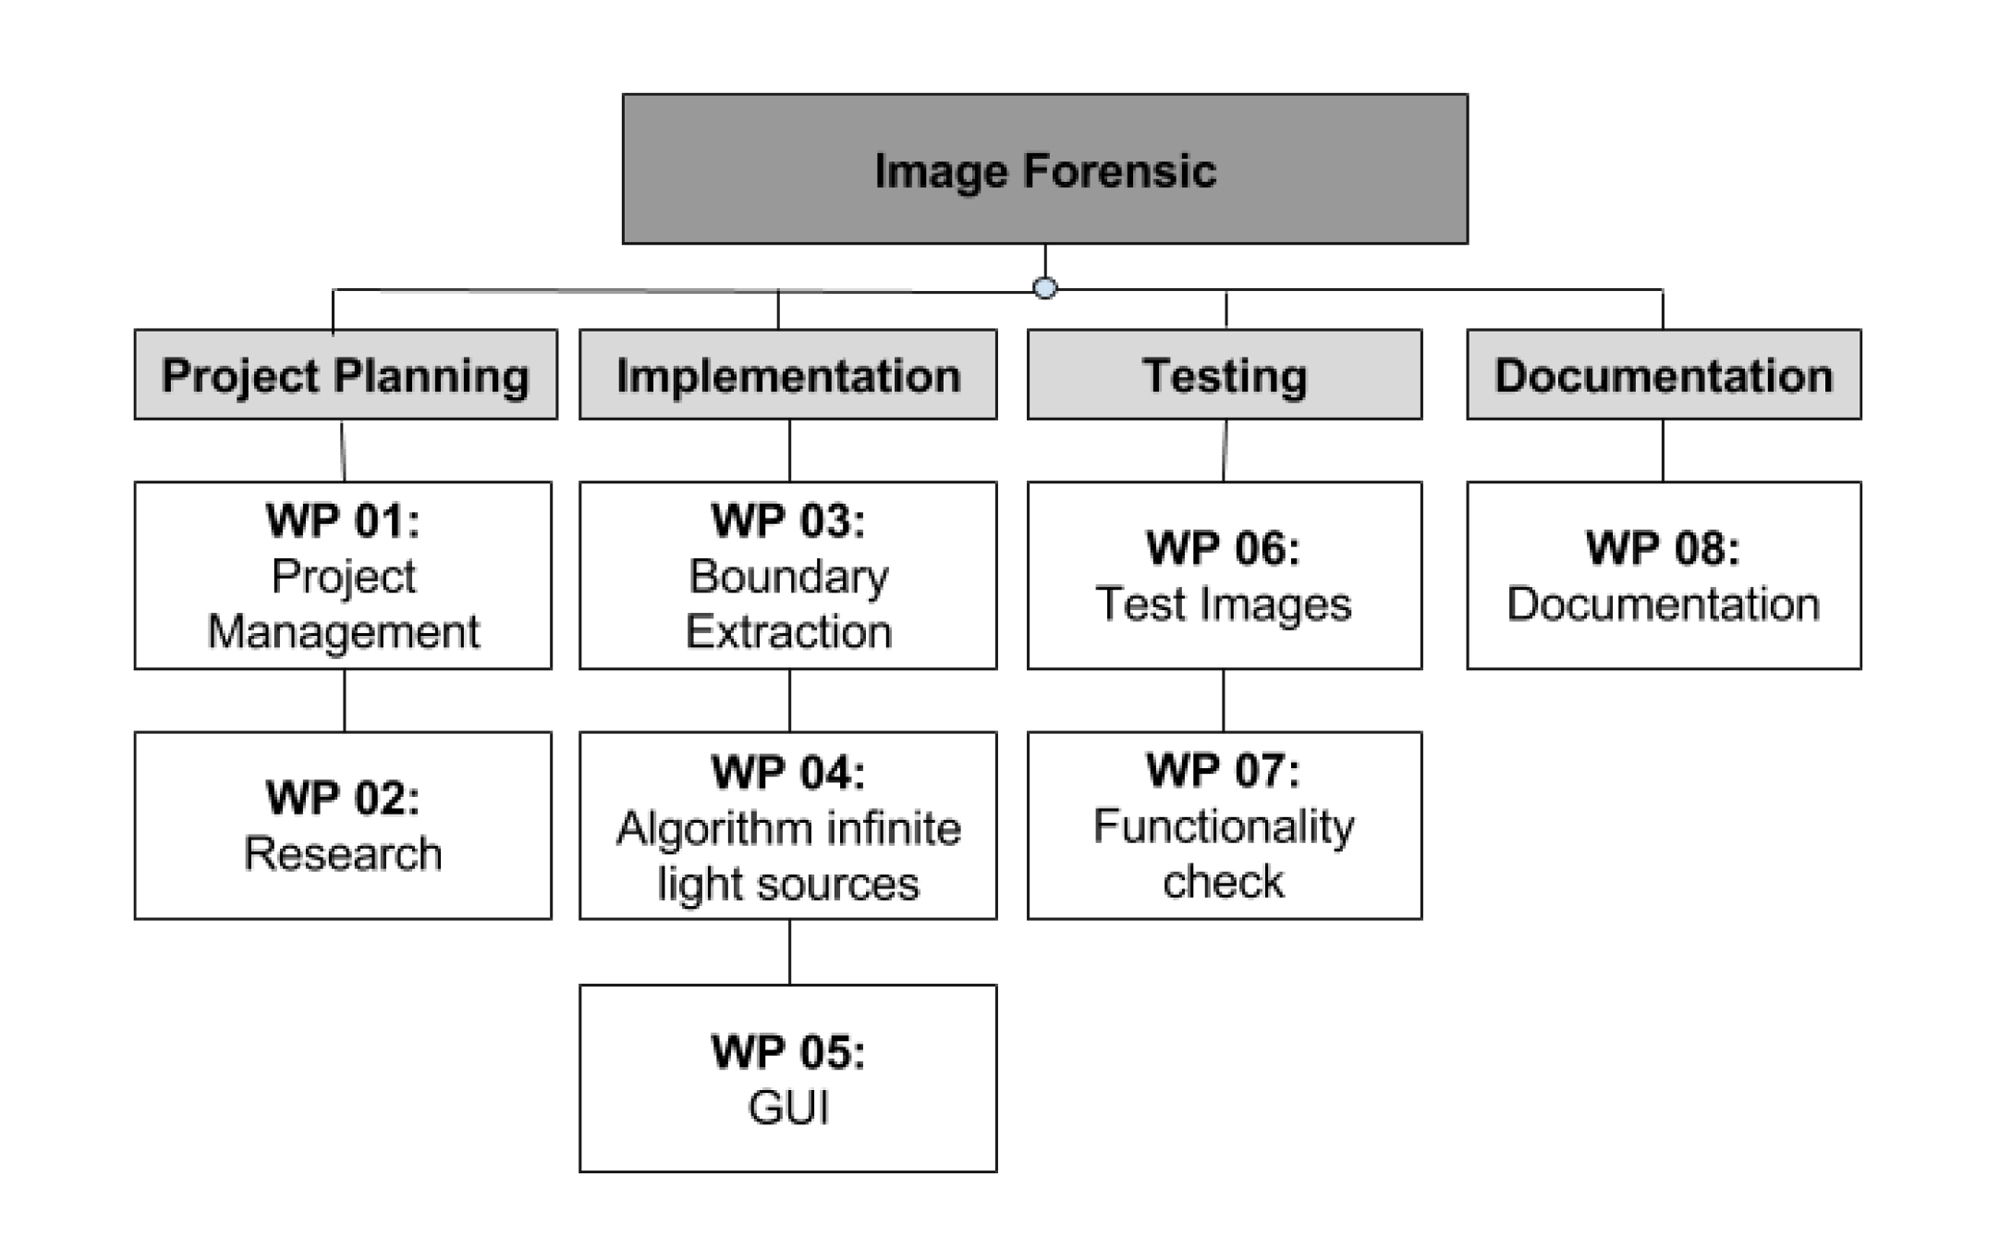
\includegraphics[scale = 0.9]{Images/Project Structure Plan.jpg}		
\end{figure}

\subsection{Milestones} \label{sec:Milestones}
\todo[inline, color=yellow]{Laura}
\begin{figure}[H] 
	\center 
	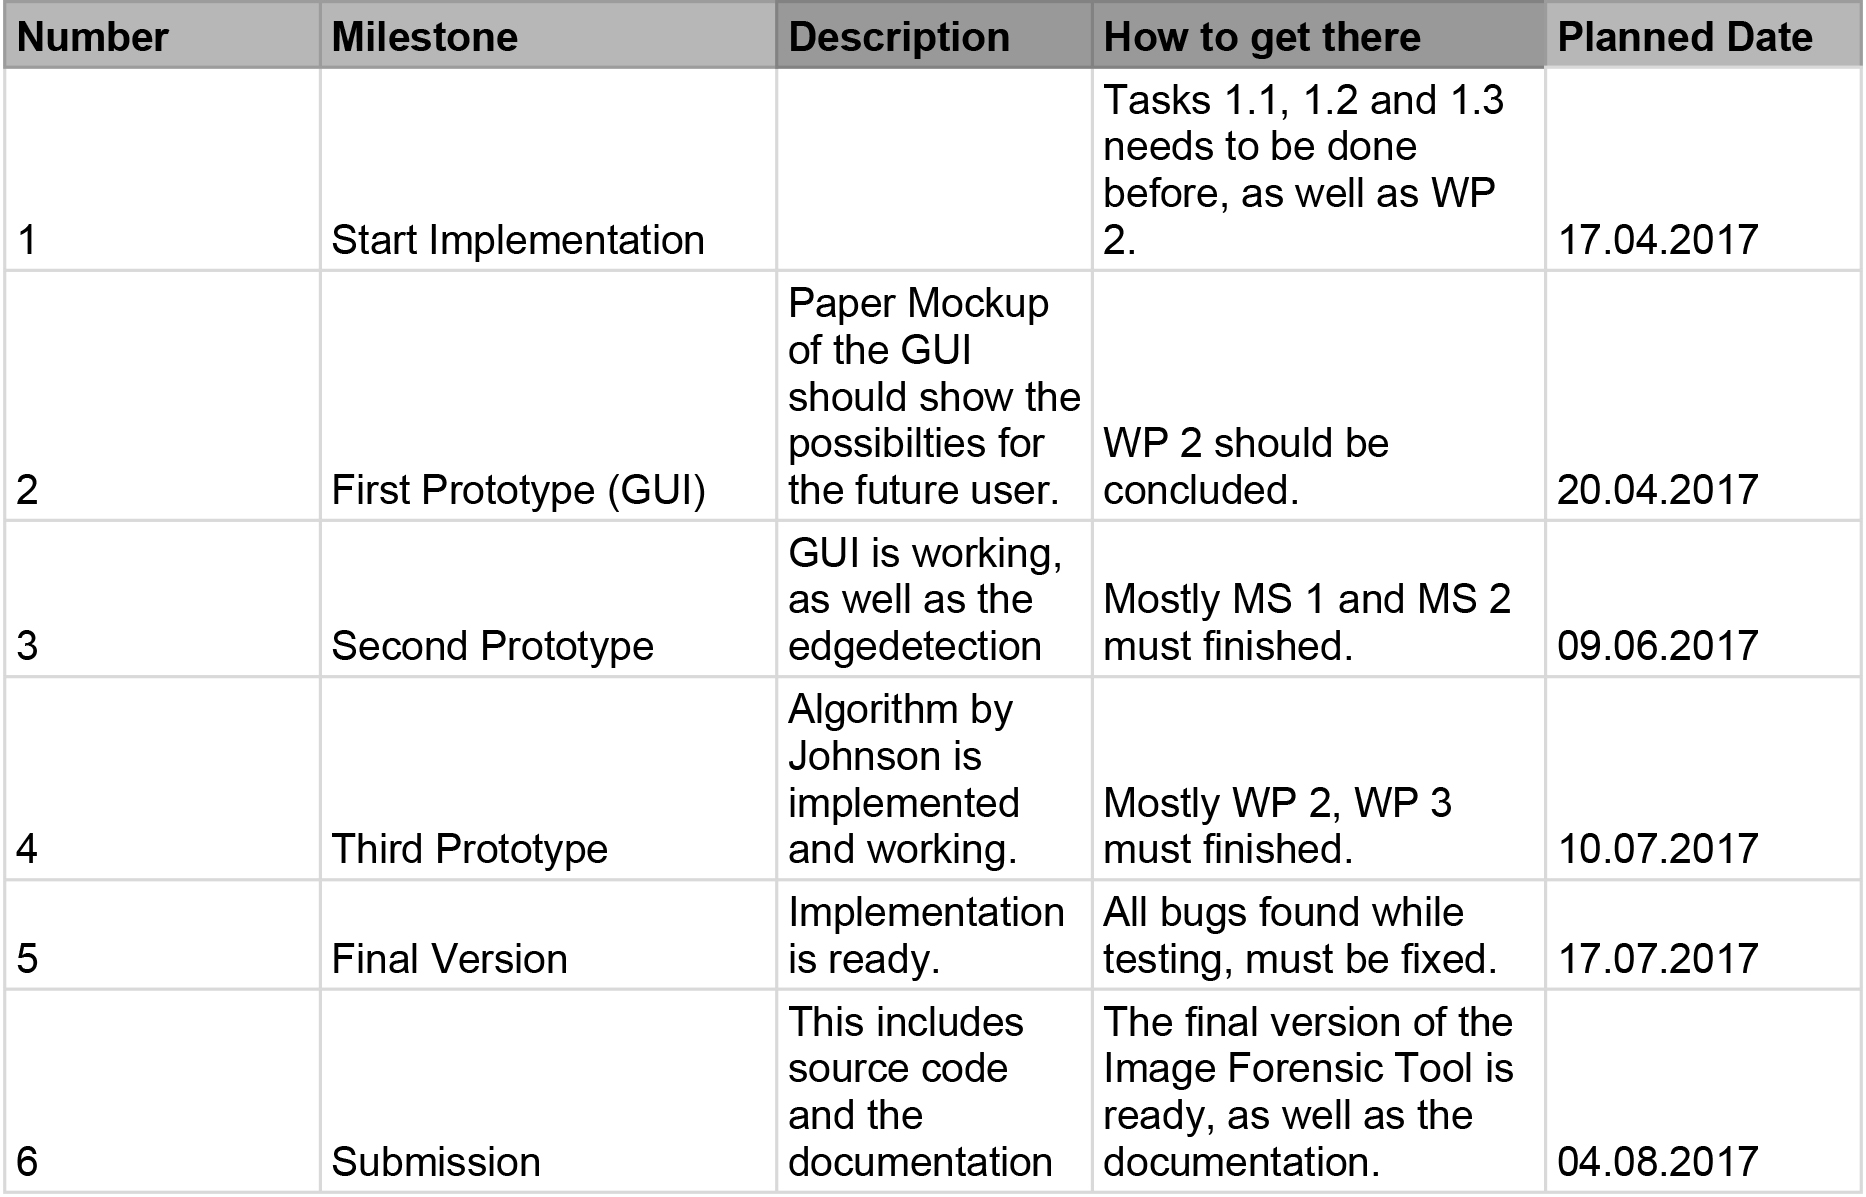
\includegraphics[scale = 0.9]{Images/milestones.jpg}		
\end{figure}
\newpage
\subsection{Time Exposure} \label{sec:timeExposure}
\todo[inline, color=yellow]{Laura}
\begin{figure}[H] 
	\center 
	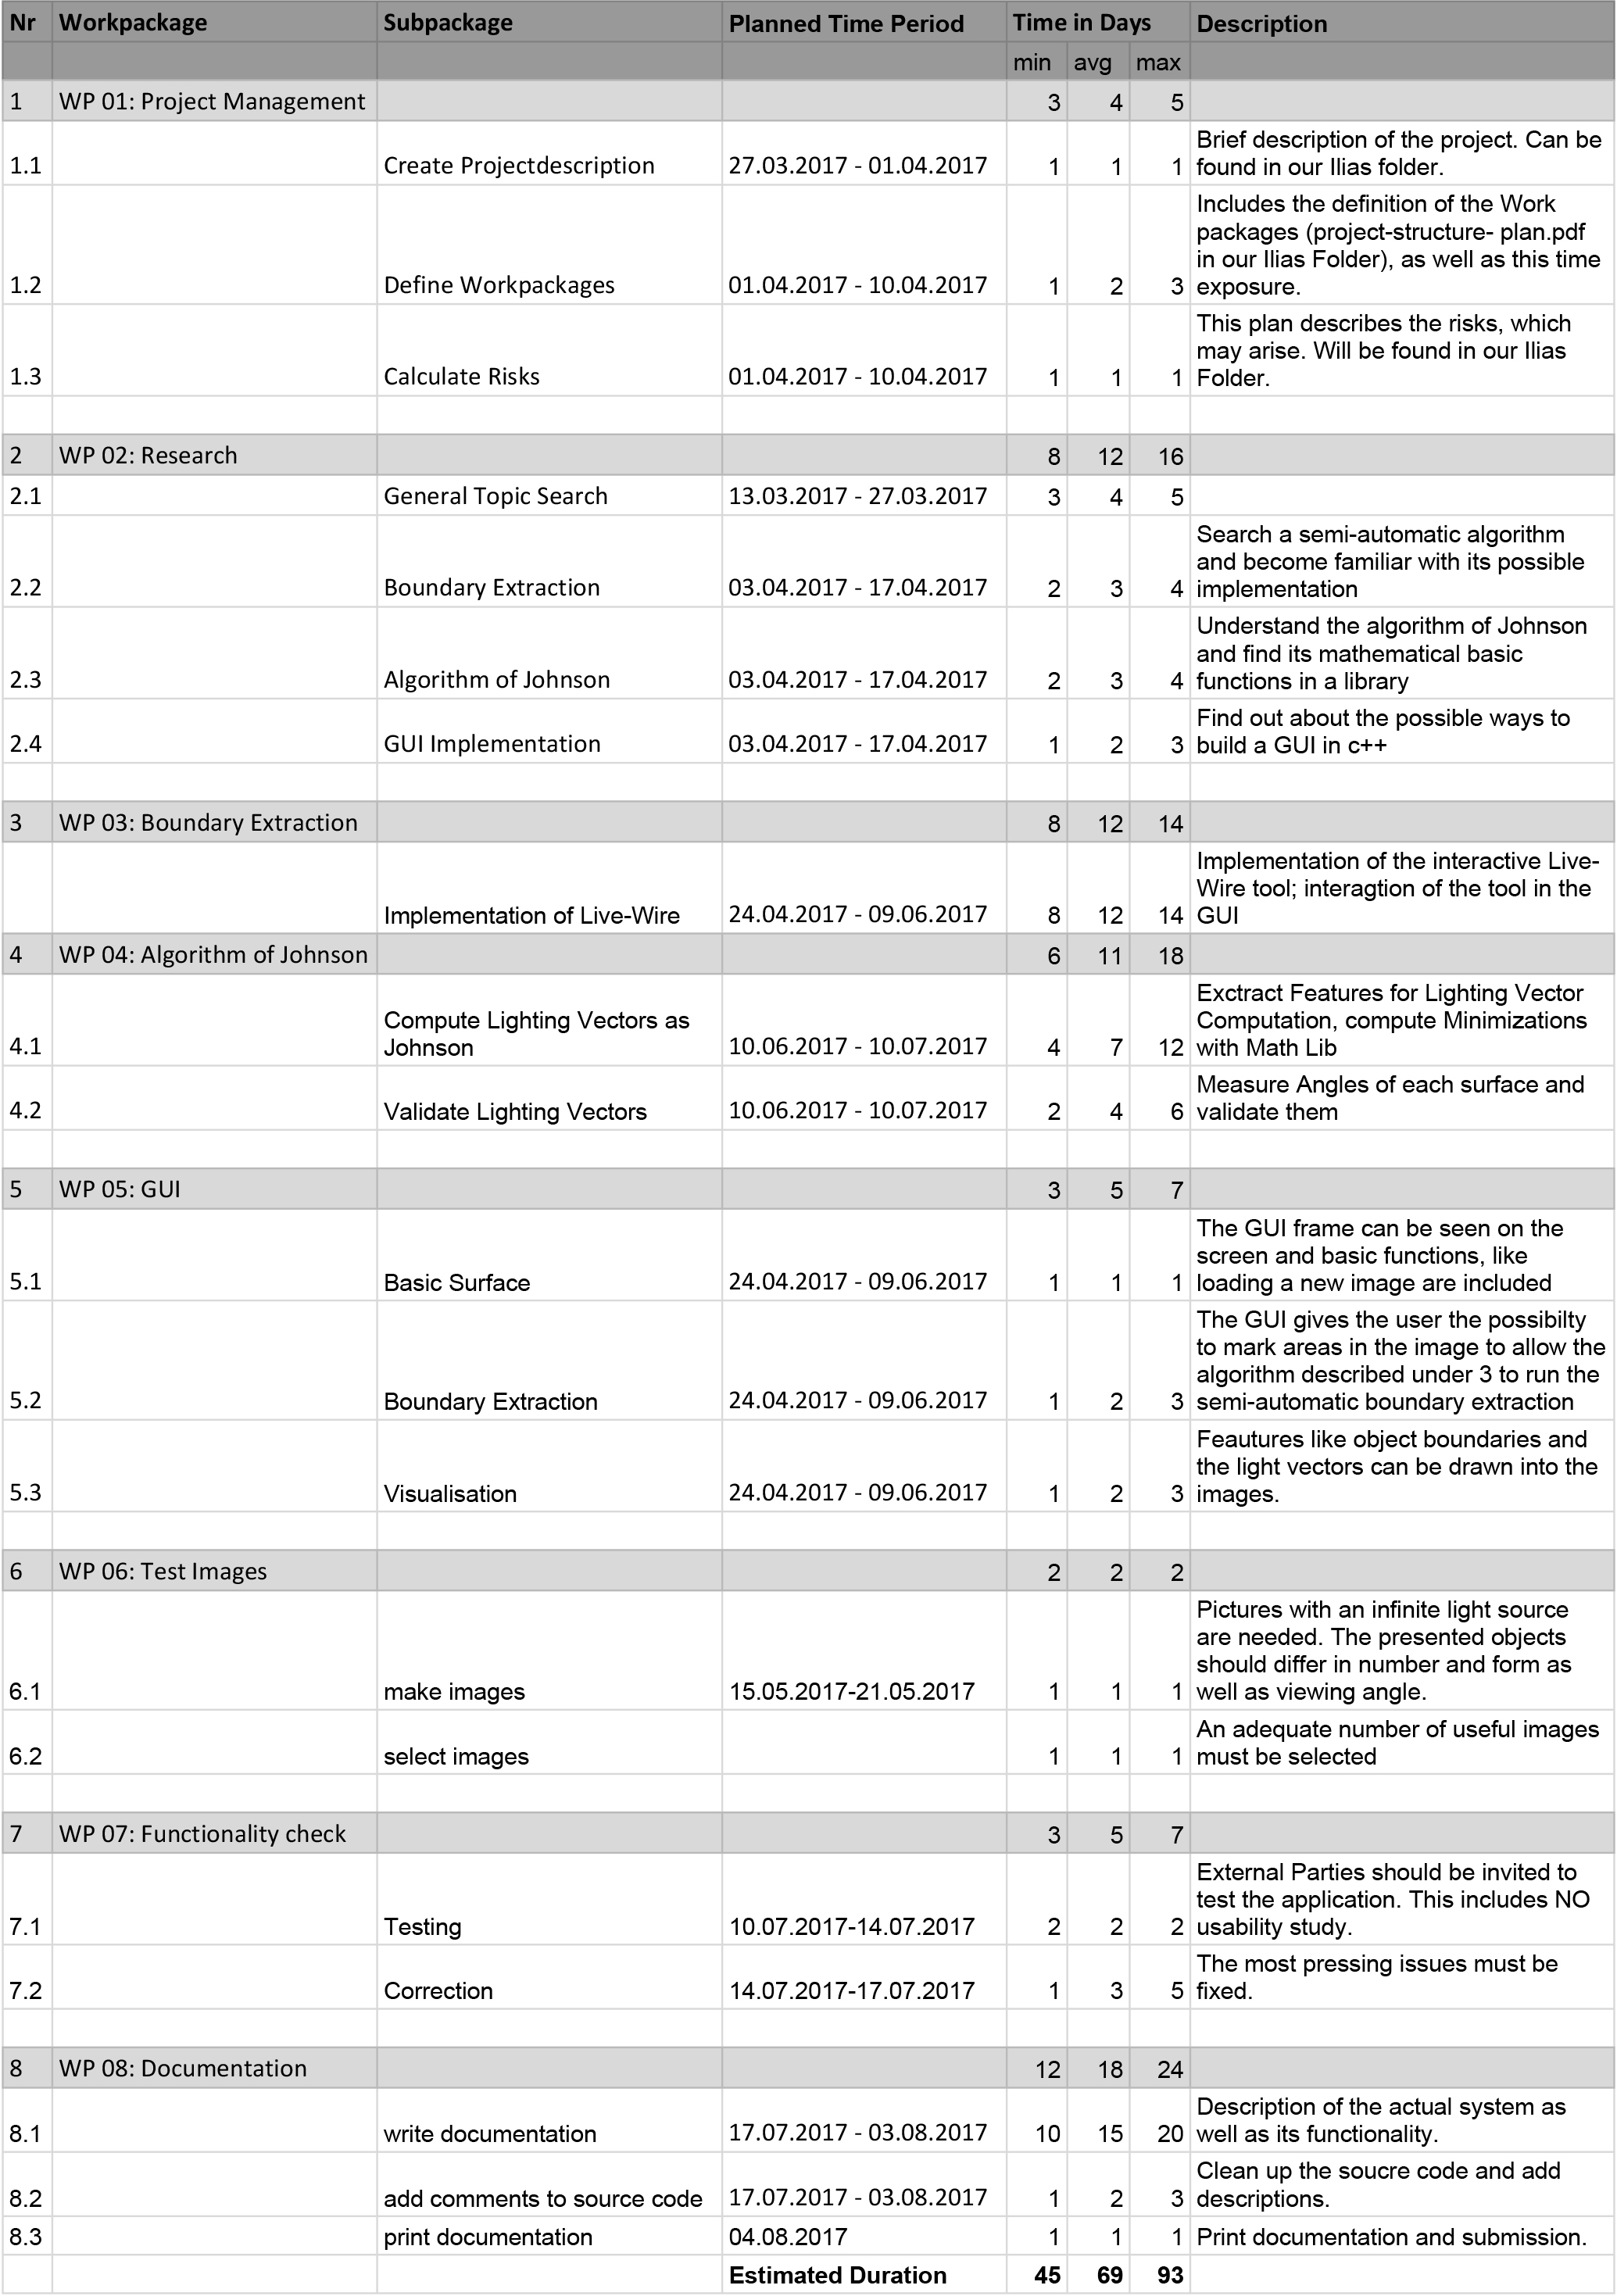
\includegraphics[scale = 0.85]{Images/Project Description and Time Exposure.jpg}		
\end{figure}



\subsection{Risks} \label{sec:risks}
\todo[inline, color=yellow]{Laura}
\begin{figure}[H] 
	\center 
	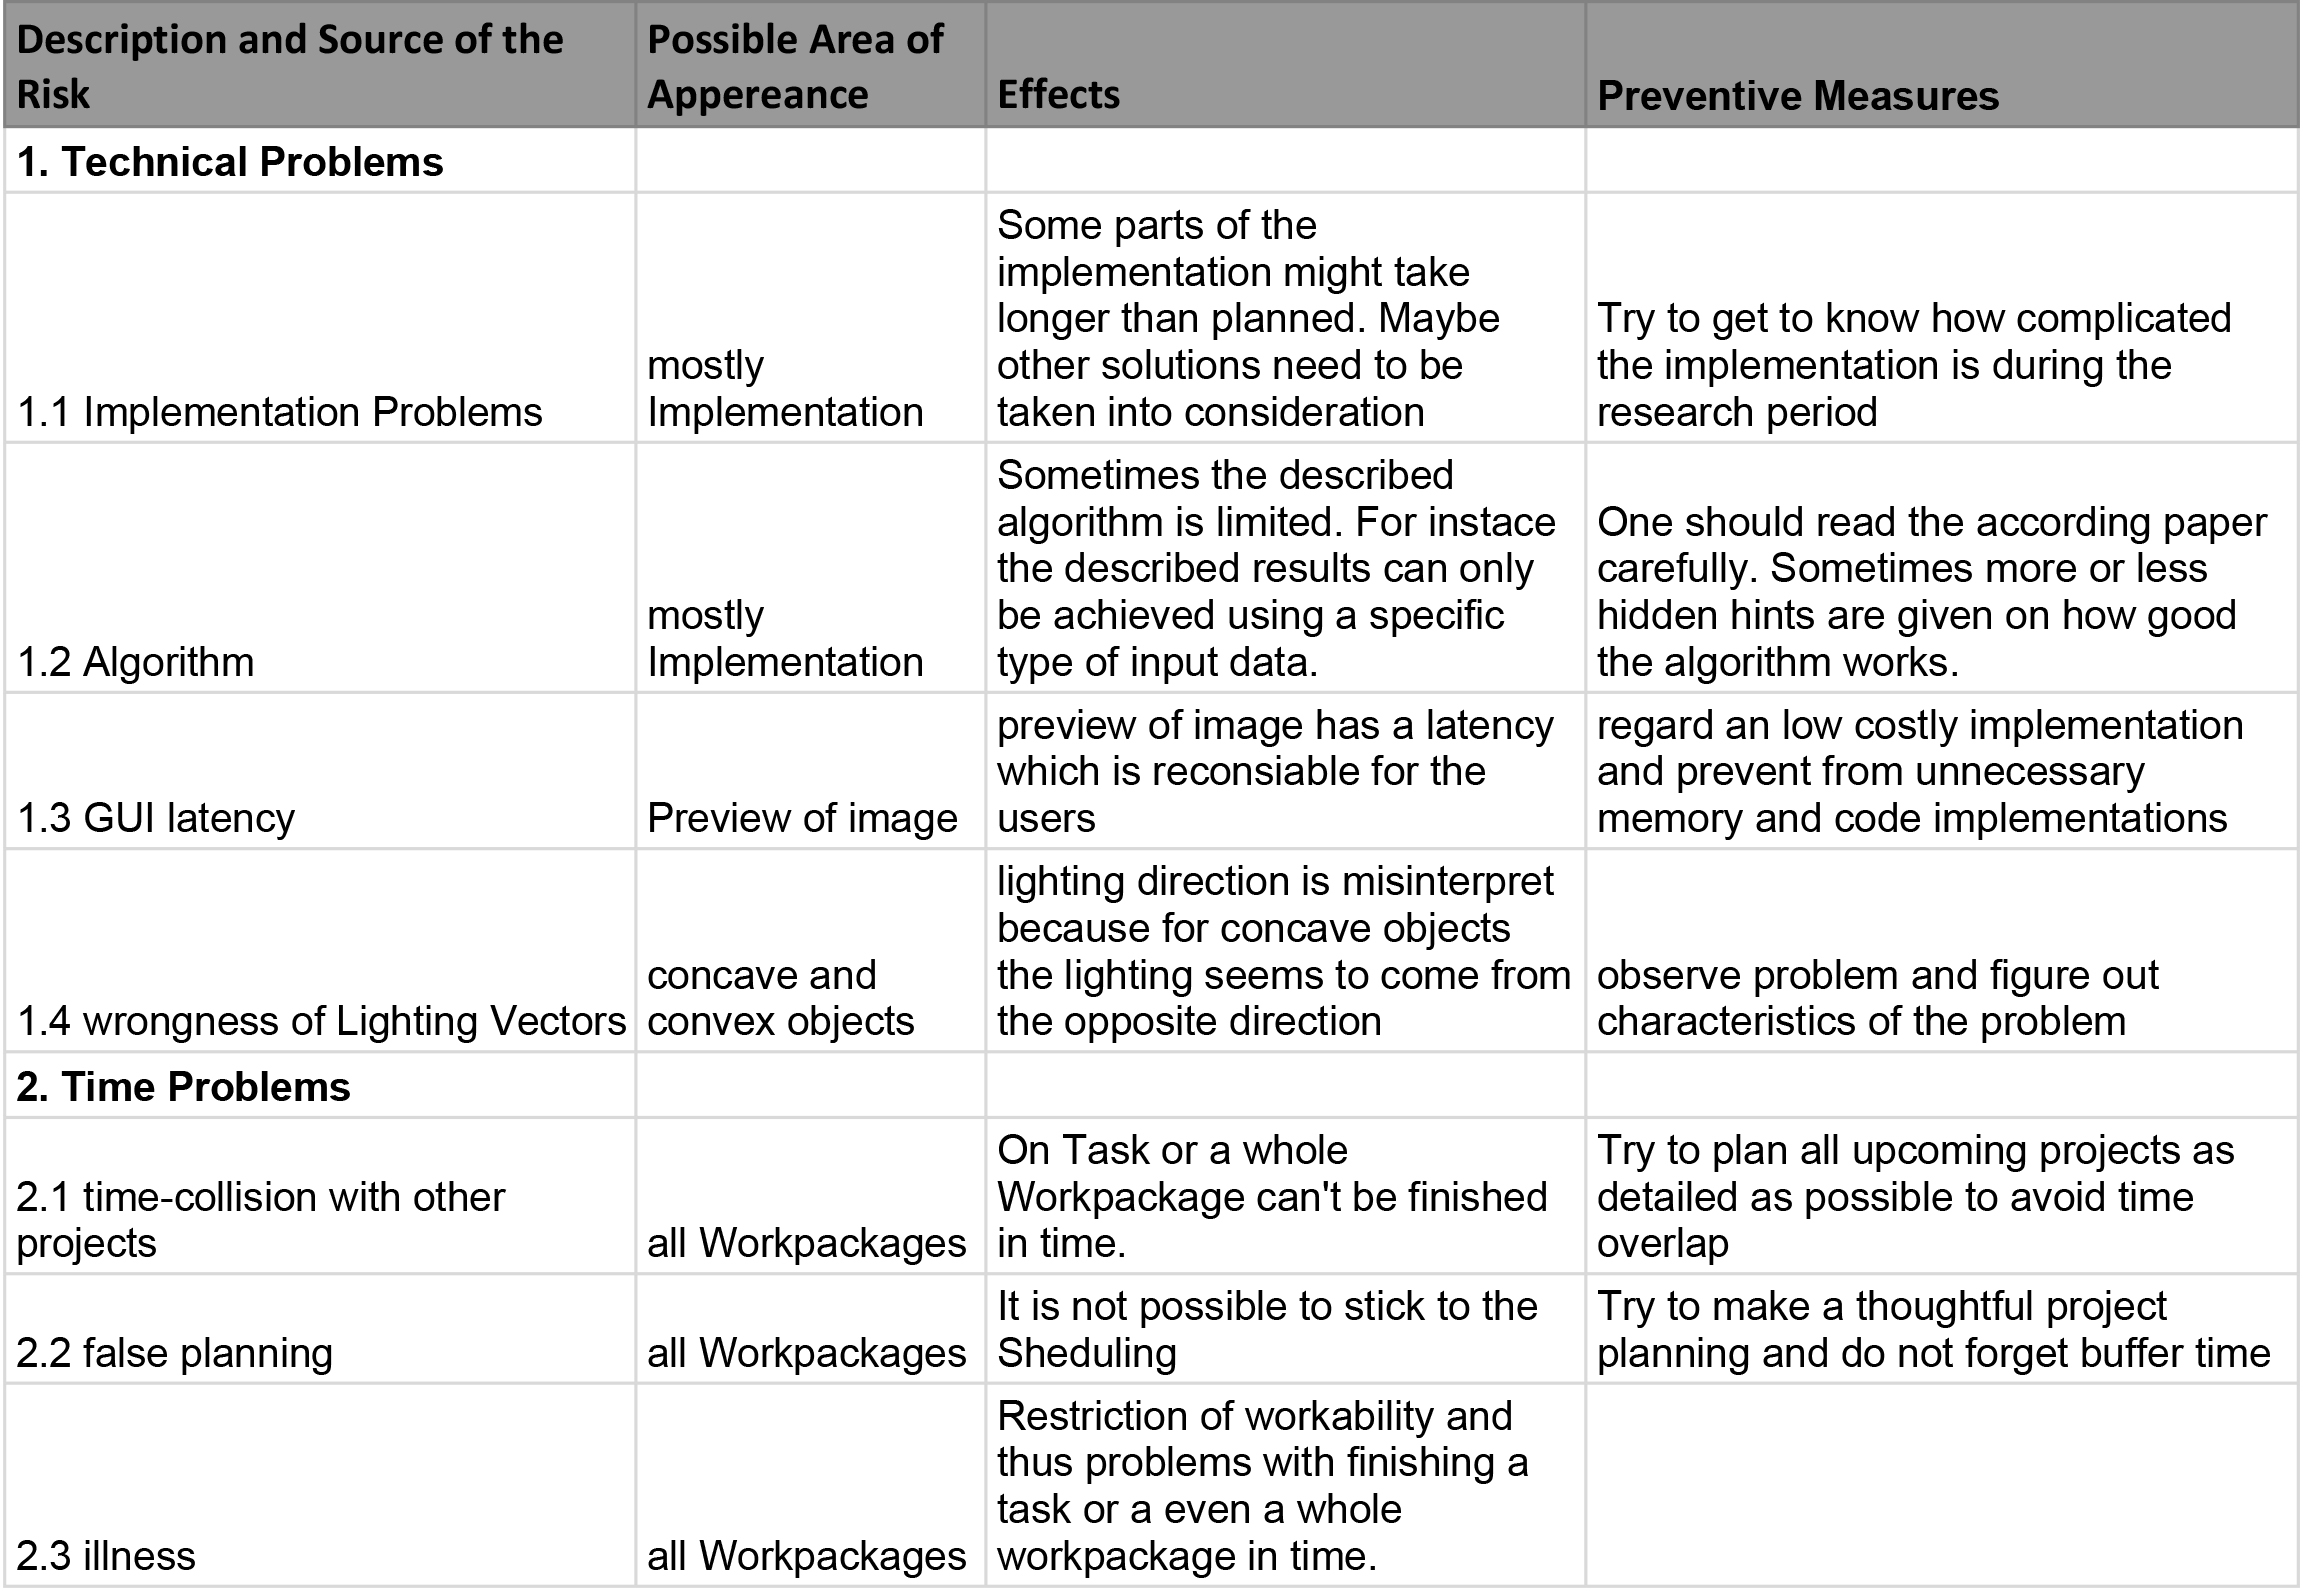
\includegraphics[scale = 0.7]{Images/risks.jpg}			
\end{figure}

\subsection{Conclusion on the Project Progress} \label{sec:pmCon}
\todo[inline, color=yellow]{Laura}
In general the project progress went well and most of the project goals were achieved. Therefore the \textit{Interactive Lighting Detector} is a complete working application. The final system contains a GUI, in which the user can select parts of the contour (compare section~\ref{sec:contours}). \\
However some of the project goals were too ambitious for the resources capacity in the scheduled time window. The planned \textit{Live Wire} algorithm was replaced by simply taking a binary mask image of the actual image and detecting the contour as described in section~\ref{sec:findContours}. In addition to that it is only possible to calculate the light vector for one object in a scene. It was planned to detect light vectors for several objects to give the opportunity of comparing the directions to each other. But nevertheless, the calculated light vector can be compared to the shadow created by the sundial. \\
The determination of the light vectors is not working as trustworthy. Reasons for that are discussed in evaluation (compare section~\ref{sec:Evaluation}) and summed up in the conclusion (compare section~\ref{sec:Conclusion}).



\newpage

























